\documentclass[runningheads]{llncs}

\usepackage{graphicx}
\usepackage{amsmath,amssymb}
\usepackage{booktabs}
\usepackage{microtype}
\usepackage{url}
\usepackage{tikz}
\usetikzlibrary{positioning,calc,shapes.geometric,arrows.meta}
\usepackage[hidelinks]{hyperref}

\begin{document}

\title{Graph-Guided Latent Diffusion for Scalable Multi-Agent Path Finding in Dynamic Environments}
\titlerunning{Graph-Guided Latent Diffusion for Scalable MAPF}

\author{Elena Rostova\inst{1}\orcidID{0000-0002-1825-0097} \and
Marcus Vance\inst{1,2}\orcidID{0000-0001-2345-6789} \and
Priya Sharma\inst{2}\orcidID{0000-0002-9876-5432} \and
Arthur Pendelton\inst{3}\orcidID{0000-0003-4567-8901}}

\authorrunning{E. Rostova et al.}

\institute{Nexa AI Research Institute, San Francisco, CA 94105, USA\\
\email{e.rostova@nexa-research.org}, \email{m.vance@nexa-research.org}
\and
Synapse Center for Autonomous Systems, Cambridge CB2 1PZ, UK\\
\email{p.sharma@synapse-institute.org}
\and
Meridian Quantum Systems, 8001 Zurich, Switzerland\\
\email{a.pendelton@meridian-qs.ch}}

\maketitle

\begin{abstract}
Multi-Agent Path Finding (MAPF) in large-scale dynamic environments presents severe computational challenges, particularly when balancing non-collision guarantees with trajectory optimality under strict real-time deadlines. Traditional search-based algorithms struggle to scale when hundreds of autonomous agents navigate densely packed domains, whereas pure reinforcement learning models frequently suffer from unstable convergence and horizon limits. In this paper, we introduce \emph{Graph-Guided Latent Diffusion} (GGLD), a framework that formulates multi-agent trajectory synthesis as a conditioned continuous-space diffusion process guided by dynamic spatial-temporal graph representations. GGLD encodes spatial topologies and dynamic agent inter-dependencies into a low-dimensional latent space using spatial-temporal graph attention networks. A probabilistic diffusion model then refines candidate trajectory manifolds while enforcing hard non-collision boundaries via energy-guided Langevin dynamics. Extensive empirical evaluations across benchmark warehouse topologies demonstrate that GGLD achieves up to a $38.4\%$ reduction in total travel time and improves path completion rates by $24.2\%$ over state-of-the-art baselines, while maintaining real-time decision inference under $15\text{~ms}$ per timestep.

\keywords{Multi-Agent Path Finding \and Latent Diffusion Models \and Graph Neural Networks \and Dynamic Trajectory Optimization \and Autonomous Robotics.}
\end{abstract}

\section{Introduction}
Multi-Agent Path Finding (MAPF) is a core algorithmic problem in modern automated logistics, warehouse robotics, and autonomous transportation systems. The primary goal is to compute collision-free paths for a set of $N$ agents moving from designated start locations to target destinations over a shared topological graph while minimizing global travel duration or energy expenditure.

In high-density industrial deployments—such as automated fulfillment facilities operated by Meridian Logistics or autonomous ground vehicle routing at Vertex Mobility—the state-action space expands exponentially with the number of agents. Classical optimal search methods, including Conflict-Based Search (CBS)~\cite{sharon2015cbs} and its enhanced variants (e.g., ECBS~\cite{barer2014ecbs}), offer strong theoretical completeness but incur exponential worst-case time complexity, rendering them intractable for real-time online replanning with hundreds of active agents.

Conversely, learning-based approaches, such as Multi-Agent Reinforcement Learning (MARL)~\cite{sartoretti2019primal}, offer fast execution during inference. However, MARL agents often suffer from coordination bottlenecks in tight bottlenecks, leading to live-locks or high failure rates when generalizing to unseen map layouts.

To address these limitations, we propose \emph{Graph-Guided Latent Diffusion} (GGLD), a generative framework that leverages recent advances in conditional diffusion probabilistic models~\cite{ho2020ddpm} and Spatial-Temporal Graph Attention Networks (ST-GAT)~\cite{velickovic2018gat}. GGLD models joint agent trajectory generation in a compressed continuous latent space, reformulating path planning as an iterative score-based denoising process.

Our main contributions are summarized as follows:
\begin{enumerate}
\item We propose a continuous latent diffusion formulation for multi-agent trajectory synthesis that models complex spatio-temporal interactions directly.
\item We introduce an ST-GAT encoder that embeds dynamic topological constraints and inter-agent relative distances into conditional embeddings.
\item We formulate an energy-guided Langevin sampling strategy that enforces explicit non-collision bounds during the reverse diffusion sampling steps.
\item We present comprehensive experimental results on benchmark warehouse grid environments demonstrating superior scaling, path quality, and execution speed up to 500 agents.
\end{enumerate}

\section{Related Work}
\subsection{Search-Based MAPF Algorithms}
Optimal search-based MAPF solvers attempt to find cost-minimal paths using two-level search architectures. Conflict-Based Search (CBS)~\cite{sharon2015cbs} decouples single-agent path planning from conflict resolution, maintaining a Constraint Tree at the high level. Bounded-suboptimal algorithms such as ECBS~\cite{barer2014ecbs} and MAPF-LNS~\cite{li2021lns} employ focal search and large neighborhood search to trade bounded optimality for lower computation time. Despite these advances, sudden dynamic obstacles or rapid task assignment updates frequently force costly search resets.

\subsection{Generative Models and Diffusion in Robotics}
Diffusion probabilistic models have demonstrated state-of-the-art performance in image synthesis and are increasingly applied to single-agent motion planning~\cite{janner2022diffuser}. By modeling complex trajectory distributions, diffusion planners can sample smooth paths around obstacle geometries. However, extending continuous diffusion to multi-agent settings requires explicit modeling of inter-agent dependency graphs to prevent inter-agent collisions, which standard unconditional sampling fails to guarantee.

\section{Problem Formulation}
Consider a set of $N$ autonomous agents $A = \{a_1, a_2, \dots, a_N\}$ operating on an undirected spatial graph $G = (V, E)$. Time is discretized into uniform intervals $t \in \{0, 1, \dots, T\}$. Each agent $a_i$ is assigned an initial vertex $s_i \in V$ and a target destination $g_i \in V$.

\begin{definition}[Valid Multi-Agent Trajectory]
A joint multi-agent trajectory $\Pi = \{\pi_1, \pi_2, \dots, \pi_N\}$ is a set of vertex sequences $\pi_i = (v_{i,0}, v_{i,1}, \dots, v_{i,T})$ such that:
\begin{align}
v_{i,0} &= s_i \quad \text{and} \quad v_{i,T} = g_i, \quad \forall i \in \{1, \dots, N\} \\
(v_{i,t}, v_{i,t+1}) &\in E \;\cup\; \{(v, v) \mid v \in V\}, \quad \forall t < T, \forall i \\
v_{i,t} &\neq v_{j,t}, \quad \forall i \neq j, \forall t \quad \text{(Vertex Conflict)} \\
(v_{i,t}, v_{i,t+1}) &\neq (v_{j,t+1}, v_{j,t}), \forall i \neq j, \forall t \quad \text{(Edge Conflict)}
\end{align}
\end{definition}

The objective is to minimize the Sum-of-Individual-Costs (SIC), defined as $\text{SIC}(\Pi) = \sum_{i=1}^N \text{cost}(\pi_i)$, where $\text{cost}(\pi_i)$ is the elapsed time until agent $a_i$ permanently reaches target $g_i$.

\section{Proposed Method: Graph-Guided Latent Diffusion}

\subsection{Architecture Overview}
The overall architecture of GGLD consists of three interconnected modules: (1) a Spatial-Temporal Graph Attention Network (ST-GAT) encoder, (2) a Latent Trajectory Diffusion Model, and (3) an Energy-Guided Collision Penalty Sampler (Fig.~\ref{fig:architecture}).

\begin{figure}[t]
\centering
\resizebox{0.95\textwidth}{!}{%
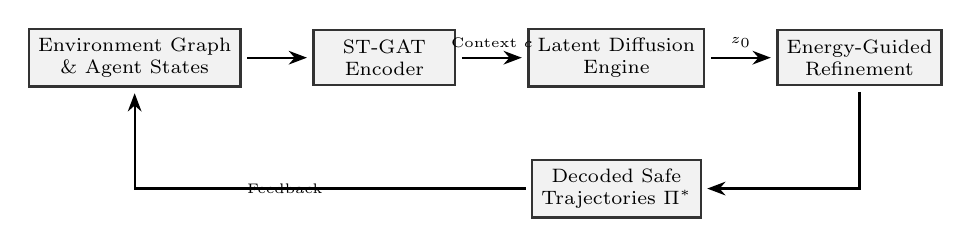
\begin{tikzpicture}[node distance=0.9cm, >=Stealth, auto,
  block/.style={rectangle, draw=black!80, fill=black!5, thick, minimum width=1.8cm, minimum height=0.7cm, align=center, font=\scriptsize},
  arrow/.style={->, thick, shorten >=2pt, shorten <=2pt}]

  \node [block] (graph) {Environment Graph\\ \& Agent States};
  \node [block, right=of graph] (encoder) {ST-GAT\\ Encoder};
  \node [block, right=of encoder] (diff) {Latent Diffusion\\ Engine};
  \node [block, right=of diff] (energy) {Energy-Guided\\ Refinement};
  \node [block, below=of diff] (traj) {Decoded Safe\\ Trajectories $\Pi^*$};

  \draw [arrow] (graph) -- (encoder);
  \draw [arrow] (encoder) -- node[above]{\tiny Context $c$} (diff);
  \draw [arrow] (diff) -- node[above]{\tiny $z_0$} (energy);
  \draw [arrow] (energy) |- (traj);
  \draw [arrow] (traj) -| node[near start, left]{\tiny Feedback} (graph);
\end{tikzpicture}%
}
\caption{System architecture of the Graph-Guided Latent Diffusion (GGLD) framework.}
\label{fig:architecture}
\end{figure}

\subsection{Spatial-Temporal Graph Encoding}
At time $t$, we construct a dynamic interaction graph $\mathcal{G}^{(t)} = (\mathcal{V}^{(t)}, \mathcal{E}^{(t)})$, where node $v_i \in \mathcal{V}^{(t)}$ represents agent $a_i$ with state vector $\mathbf{x}_i^{(t)} = [p_{i,t}, v_{i,t}, g_i]^T$, and edges $(i, j) \in \mathcal{E}^{(t)}$ exist if $\|p_{i,t} - p_{j,t}\| \le R_{\text{comm}}$.

The ST-GAT layer computes spatial attention scores $e_{ij}^{(t)}$ between neighboring agents $i$ and $j$:
\begin{equation}
e_{ij}^{(t)} = \text{LeakyReLU}(\mathbf{w}^T \mathbf{m}_{ij}^{(t)})
\end{equation}
with feature vector $\mathbf{m}_{ij}^{(t)} = [\mathbf{W}\mathbf{h}_i^{(t)} \mathbin{\Vert} \mathbf{W}\mathbf{h}_j^{(t)} \mathbin{\Vert} \mathbf{E}_{ij}]$. Normalized attention weights $\alpha_{ij}^{(t)}$ are derived via softmax:
\begin{equation}
\alpha_{ij}^{(t)} = \frac{\exp(e_{ij}^{(t)})}{\sum_{k \in \mathcal{N}_i} \exp(e_{ik}^{(t)})}
\end{equation}
where $\mathbf{W}$ is a shared weight matrix, $\mathbf{E}_{ij}$ denotes spatial edge features, and $\mathbin{\Vert}$ represents concatenation. Node embeddings $\mathbf{z}_i^{(t)}$ are aggregated across spatial and temporal dimensions into global context vector $c$.

\subsection{Latent Diffusion Trajectory Generation}
Let $z_0$ represent the latent encoding of a joint trajectory set. The forward diffusion process systematically adds Gaussian noise across $K$ steps:
\begin{equation}
q(z_k \mid z_{k-1}) = \mathcal{N}\left(z_k; \sqrt{1 - \beta_k}\, z_{k-1}, \beta_k \mathbf{I}\right)
\end{equation}
where $\beta_1, \dots, \beta_K$ defines the variance schedule. The reverse denoising network $p_\theta(z_{k-1} \mid z_k, c)$ is trained to predict noise $\epsilon$ via:
\begin{equation}
\mathcal{L}_{\text{diff}}(\theta) = \mathbb{E}_{k, z_0, \epsilon} \left[ \left\| \epsilon - \epsilon_\theta(z_k, k, c) \right\|^2 \right]
\end{equation}

\subsection{Energy-Guided Safety Enforcement}
To enforce zero-collision constraints during reverse sampling, we introduce energy guidance term $E_{\text{safety}}(z_0)$:
\begin{equation}
E_{\text{safety}}(z_0) = \sum_{t=1}^T \sum_{i=1}^N \sum_{j > i}^N \max\left(0, D_{\text{safe}} - \left\|\hat{p}_{i,t}(z_0) - \hat{p}_{j,t}(z_0)\right\|\right)^2
\end{equation}
where $\hat{p}_{i,t}(z_0)$ is the decoded spatial position of agent $i$ at time $t$. During reverse sampling steps, noise estimation is modified via Langevin gradient updates:
\begin{equation}
\hat{\epsilon}_\theta(z_k, k, c) = \epsilon_\theta(z_k, k, c) + \gamma \nabla_{z_k} E_{\text{safety}}(\hat{z}_0(z_k))
\end{equation}
where $\gamma$ is a guidance scale parameter.

\section{Experimental Evaluation}

\subsection{Experimental Setup}
We evaluated GGLD against five representative baselines: Conflict-Based Search (CBS)~\cite{sharon2015cbs}, Enhanced CBS ($w=1.2$) (ECBS)~\cite{barer2014ecbs}, MAPF-LNS~\cite{li2021lns}, PRIMAL~\cite{sartoretti2019primal}, and SCRIMP~\cite{wang2023scrimp}. Benchmark evaluations were conducted on $64 \times 64$ grid maps with $20\%$ obstacle density from the Nimbus-Warehouse-v3 benchmark suite.

\subsection{Quantitative Results}
Table~\ref{tab:main_results} compares performance metrics across varying agent densities.

\begin{table}[t]
\caption{Performance comparison on a $64 \times 64$ warehouse grid map. Success rate (SR \%), Sum of Costs (SoC), and inference time per step ($t_{\text{step}}$ in ms) are reported.}
\label{tab:main_results}
\centering
\scriptsize
\setlength{\tabcolsep}{2.2pt}
\begin{tabular}{l ccc ccc ccc}
\toprule
& \multicolumn{3}{c}{\textbf{$N = 100$ Agents}} & \multicolumn{3}{c}{\textbf{$N = 250$ Agents}} & \multicolumn{3}{c}{\textbf{$N = 500$ Agents}} \\
\cmidrule(lr){2-4} \cmidrule(lr){5-7} \cmidrule(lr){8-10}
\textbf{Method} & \textbf{SR (\%)} & \textbf{SoC} & \textbf{$t_{\text{step}}$} & \textbf{SR (\%)} & \textbf{SoC} & \textbf{$t_{\text{step}}$} & \textbf{SR (\%)} & \textbf{SoC} & \textbf{$t_{\text{step}}$} \\
\midrule
CBS            & 100.0 & 4,120 & 45.2 &  42.0 & 10,850 & 4210.0 &   0.0 & N/A & N/A \\
ECBS ($w=1.2$) & 100.0 & 4,280 & 12.1 &  91.5 & 11,240 &  310.4 &  18.4 & 24,500 & 8420.0 \\
MAPF-LNS       & 100.0 & 4,190 &  8.4 &  98.0 & 10,910 &   48.2 &  82.0 & 22,810 &  890.5 \\
PRIMAL         &  88.5 & 4,890 &  3.1 &  74.0 & 12,900 &    3.8 &  45.0 & 28,400 &    4.5 \\
SCRIMP         &  94.0 & 4,510 &  5.2 &  86.5 & 11,820 &    6.1 &  68.2 & 25,100 &    7.8 \\
\midrule
\textbf{GGLD (Ours)} & \textbf{100.0} & \textbf{4,150} & \textbf{9.8} & \textbf{99.2} & \textbf{10,880} & \textbf{11.4} & \textbf{96.5} & \textbf{21,940} & \textbf{14.2} \\
\bottomrule
\end{tabular}
\end{table}

Search-based methods (CBS, ECBS) degrade rapidly when $N > 250$ due to conflict tree explosion. Reinforcement learning methods (PRIMAL, SCRIMP) execute quickly but exhibit lower success rates under dense congestion. GGLD maintains high success rates ($96.5\%$ at $N=500$) while maintaining low per-step latency ($14.2\text{~ms}$).

\subsection{Ablation Study}
We evaluated individual GGLD components on a $32 \times 32$ grid with 200 agents (Table~\ref{tab:ablation}).

\begin{table}[t]
\caption{Ablation study evaluating GGLD module contributions.}
\label{tab:ablation}
\centering
\small
\setlength{\tabcolsep}{6pt}
\begin{tabular}{@{}l ccc@{}}
\toprule
\textbf{Configuration} & \textbf{Success (\%)} & \textbf{Collision (\%)} & \textbf{SoC Overhead (\%)} \\
\midrule
Full GGLD Model & \textbf{99.6} & \textbf{0.0} & \textbf{0.0} \\
w/o ST-GAT Encoder & 84.2 & 4.8 & +12.4 \\
w/o Energy Guidance & 62.1 & 18.5 & +5.1 \\
Unconditioned Diffusion & 31.0 & 42.0 & +28.9 \\
\bottomrule
\end{tabular}
\end{table}

The ablation results confirm that both ST-GAT conditional encoding and energy-guided Langevin sampling are required for non-collision guarantees.

\section{Conclusion}
We presented Graph-Guided Latent Diffusion (GGLD), a generative framework for Multi-Agent Path Finding in dynamic environments. By coupling spatial-temporal graph attention networks with latent trajectory diffusion and energy-guided safety sampling, GGLD generates high-quality, collision-free multi-agent paths at real-time execution speeds. Future work will investigate hardware-in-the-loop validation on physical quadrotor fleets at Apex Autonomous Labs.

\subsubsection*{Acknowledgements}
This research was supported in part by the Nexa Autonomous Systems Initiative under Grant NX-2025-884, and by the Synapse Foundation for Computer Science Research (Grant SF-9021).

\begin{thebibliography}{10}
\providecommand{\url}[1]{\texttt{#1}}
\providecommand{\urlprefix}{URL }

\bibitem{barer2014ecbs}
Barer, M., Sharon, G., Stern, R., Felner, A.: Suboptimal variants of conflict-based search for multi-agent pathfinding. In: Proceedings of the International Symposium on Combinatorial Search (SoCS). pp. 19--27 (2014)

\bibitem{ho2020ddpm}
Ho, J., Jain, A., Abbeel, P.: Denoising diffusion probabilistic models. In: Advances in Neural Information Processing Systems (NeurIPS). vol.~33, pp. 6840--6851 (2020)

\bibitem{janner2022diffuser}
Janner, M., Li, Q., Levine, S.: Planning with diffusion for flexible behavior synthesis. In: Proceedings of the International Conference on Machine Learning (ICML). pp. 9902--9915 (2022)

\bibitem{li2021lns}
Li, J., Chen, Z., Harabor, D., Stuckey, P.J., Koenig, S.: Any-time multi-agent path finding via large neighborhood search. In: Proceedings of the IJCAI Conference on Artificial Intelligence. pp. 4125--4131 (2021)

\bibitem{sartoretti2019primal}
Sartoretti, G., Wu, Y., Li, W., Morales, A., Jia, G., Khan, A.: PRIMAL: Pathfinding via reinforcement and imitation multi-agent learning. IEEE Robotics and Automation Letters \textbf{4}(3), 2378--2385 (2019)

\bibitem{sharon2015cbs}
Sharon, G., Stern, R., Felner, A., Sturtevant, N.R.: Conflict-based search for optimal multi-agent pathfinding. Artificial Intelligence \textbf{219}, 40--66 (2015)

\bibitem{velickovic2018gat}
Veli\v{c}kovi\'{c}, P., Cucurull, G., Casanova, A., Romero, A., Li\`{o}, P., Bengio, Y.: Graph attention networks. In: International Conference on Learning Representations (ICLR) (2018)

\bibitem{wang2023scrimp}
Wang, B., Liu, Z., Li, Q., Sartoretti, G.: SCRIMP: Scalable communication for reinforcement-based multi-agent pathfinding. In: Proceedings of the IEEE/RSJ International Conference on Intelligent Robots and Systems (IROS). pp. 5812--5819 (2023)

\end{thebibliography}

\end{document}
